\documentclass{article}

\usepackage[letterpaper,top=2cm,bottom=2cm,left=3cm,right=3cm,marginparwidth=1.75cm]{geometry}

\usepackage[english]{babel}
\usepackage{amsmath}
\usepackage{setspace}
\usepackage{graphicx}
\usepackage{import}
\usepackage{natbib}
%\usepackage{lineno}
\usepackage{url}
\usepackage{xr-hyper}
\usepackage[hidelinks]{hyperref}
\usepackage{booktabs}
\usepackage{authblk}
\usepackage{float}
\usepackage{xcite}
\usepackage{xcolor}
\usepackage[font=footnotesize, labelfont=bf]{caption}

% ---------------------------------------------------------------

\title{Global poverty estimation using private and public sector big data sources}

\author[1]{Robert Marty}
\author[1]{Alice Duhaut$^{*}$}

\affil[1]{World Bank}

\renewcommand\Authands{ and }

\begin{document}


\maketitle

\bigskip

\begin{table}
    \centering
    \small
    \begin{tabular}{p{2.2cm} ll p{7.0cm}}
    \hline
    Source & Time Span & Level/Change & Features for Poverty Estimation \\
    \hline
    \multicolumn{3}{l}{\bf Daytime and Nighttime Satellite Imagery} \\
    VIIRS & 2012-  Present & Level & Nighttime lights: Average, standard deviation over time, and standard deviation over space \\
    
    \addlinespace[1ex]
    Harmonized DMSP-OLS and VIIRS & 1992 - 2021 & Changes & Nighttime Lights: Average and standard deviation over space \\
    
    \addlinespace[1ex]
    Landsat 7 & 1999 - 2021 & Both & Spectral bands and indices (NDVI and build-up index): Average, standard deviation over time, and standard deviation over space \\
    
    \addlinespace[1ex]
    - & - & Changes & Convolutional neural network used to train daytime imagery on nighttime lights; features from CNN extracted \\
    
    \addlinespace[1ex]
    Sentinel-2 & 2015 - Present & Levels & Convolutional neural network used to train daytime imagery on nighttime lights; features from CNN extracted \\

    \addlinespace[1ex]
    \color{red}MOSAIKS & \color{red}2019 & \color{red}Levels & \color{red} Features extracted from high resolution daytime imagery \\
    \hline  
    \multicolumn{3}{l}{\bf Synthetic Aperture Radar Data} \\
    Sentinel-1 & 2014 - Present & Levels & Synthetic aperture radar data, measuring average and standard deviation of VV and VH signals, and the ratio of the two---VV/VH. VV indicates vertical transmit, vertical receive, and VH indicates vertical transmit, horizontal receive. \\
    
    \hline
    \multicolumn{3}{l}{\bf Facebook Marketing Data} \\
    Facebook & Present & Levels & Proportion of monthly active Facebook users according to select attributes (e.g., proportion of Facebook users with an iPhone) \\
    
    \hline
    \multicolumn{3}{l}{\bf Roads and Points of Interest} \\
    OpenStreetMap & Present & Levels & (1) Number of points of interests (POIs) near survey (all and by type---e.g., restaurants, schools, health facilities, etc), (2) distance to nearest POI (all and by type), (3) Length of roads near survey (all and by type---e.g., trunk roads, primary roads, etc), and (4) distance to nearest road (all and by type) \\
    
    \hline
    \multicolumn{3}{l}{\bf Land Cover and Type} \\
    ESA-GlobCover & 1992-2018 & Both & Proportion of area near survey classified according to 36 different land cover classes \\

    \addlinespace[1ex]
   Shuttle Radar Topography Mission (SRTM) & Time-Invariant & Levels & Average elevation and slope \\

    \hline
    \multicolumn{3}{l}{\bf Weather and Climate} \\
    % https://www.worldclim.org/data/worldclim21.html
    WorldClim & Average of 1970-2000 & Levels & 19 bioclimatic variables, including annual mean temperature, annual precipitation, mean temperature of wettest quarter, etc. \\
    
    \addlinespace[1ex]
    % https://developers.google.com/earth-engine/datasets/catalog/ECMWF_ERA5_DAILY?hl=en#bands
    European Centre for Medium-Range Weather Forecasts: ERA5 & 1979-2020 & Both & Average annual precipitation and temperature \\
    
    \hline
    \multicolumn{3}{l}{\bf Pollution} \\
    Sentinel-5P & 2018 - Present & Levels & Average pollution levels from six metrics: nitrogen dioxide, carbon monoxide, sulphur dioxide, ozone, formaldehyde, and an aerosol index.  \\ 
    
    \addlinespace[1ex]
    MODIS & 2000 - Present & Both & Aerosol optical depth \\
    
    \hline
    \end{tabular}
    \caption{Summary of data sources for poverty estimation.}
    \label{tab:dataset_source}
\end{table}

\begin{figure}[H]
    \centering
    \includegraphics[width=1\textwidth]{figures/cor_all_fb_osm.png}
    \caption{Distribution of within-country correlations of select variables to levels of wealth. Correlations are computed at the cluster level using the latest survey year for each country. {\bf Panel A} shows the distribution of within-country correlations of the feature with the highest median correlation across countries for each dataset. {\bf Panel B} shows the correlation of all variables from the Facebook marketing data. {\bf Panel C} shows select variables from OpenStreetMap data; the panel shows all variables of (1) the length of different classes of roads and (2) the number of different points of interests (POIs) near survey clusters. {\bf Panel D} shows the correlation of all pollution variables from Sentinel-5P and MODIS; AOD variables are from MODIS and the other variables are from Sentinel-5P. The boxplots include: center line, median; box limits, upper and lower quartiles; whiskers, 1.5x interquartile range; points beyond whiskers, outliers.}
     \label{fig:cor_levels}
\end{figure}

\begin{figure}[H]
    \centering
    \includegraphics[width=1\textwidth]{figures/cor_changes.png}
    \caption{Distribution of within-country correlation of changes in select variables to changes in wealth, using clusters as the unit of analysis. We show the two variables with the highest median correlation for each dataset. The boxplots include: center line, median; box limits, upper and lower quartiles; whiskers, 1.5x interquartile range; points beyond whiskers, outliers.}
     \label{fig:cor_changes}
\end{figure}

\begin{figure}[H]
    \centering
    \includegraphics[width=1\textwidth]{figures/performence_country_avg_types.png}
    \caption{Distribution of model performance across countries, explaining levels of wealth. The black number shows the median and the red numbers show the \textcolor{black}{minimum and maximum} $r^2$. {\bf Panel A} shows model performance by the sample used to train countries. {\bf Panel B} shows model performance when using different sets of features to train models. {\bf Panel C} shows the distribution of model performance at the village and district level. Panels B and C show results where models for each country are trained on data from all other countries (the global training sample approach). The boxplots include: center line, median; box limits, upper and lower quartiles; whiskers, 1.5x interquartile range; points beyond whiskers, outliers.}
     \label{fig:performence_country_avg_types}
\end{figure}

\begin{figure}[H]
    \centering
    \includegraphics[width=1\textwidth]{figures/global_scatter_map.png}
    \caption{Performance of models predicting levels of wealth index. {\bf Panel A} shows a scatterplot of the estimated and true wealth indices. {\bf Panel B} shows model performance when considering individual countries. {\bf Panel C} and {\bf Panel D} are similar to panels A and B, but using results aggregated at the district level. All panels use results where models for each country are trained on data from all other countries (the global training sample approach). \textcolor{black}{ $r^2$ is the squared Pearson correlation coefficient, and $R^2$ is the coefficient of determination. The maps in panels B and D were produced using R, version 4.2.2 (\url{https://www.r-project.org/}); data to produce the country-level basemaps come from Natural Earth (\url{https://www.naturalearthdata.com/}).}}
     \label{fig:scatter_map}
\end{figure}

\begin{figure}[H]
    \centering
    \includegraphics[width=1\textwidth]{figures/explain_var_in_r2.png}
    \caption{Determinants of the variation in model performance across countries, explaining levels of wealth. {\bf Panel A} shows the association between GDP per capita and model performance. {\bf Panel B} shows the association between the wealth index standard deviation and model performance. {\bf Panel C} shows the association between the nighttime lights standard deviation and model performance. {\bf Panel D} shows the association between the proportion of the population on Facebook---measured using monthly active users divided by a country's population---and model performance using only Facebook features to train the model. {\bf Panel E} shows the distribution of model performance by income level using models trained across different feature sets. The boxplots include: center line, median; box limits, upper and lower quartiles; whiskers, 1.5x interquartile range; points beyond whiskers, outliers. All panels use results where models for each country are trained on data from all other countries (the global training sample approach), and where the unit of analysis is clusters.}
     \label{fig:explain_var_in_r2}
\end{figure}

\begin{figure}[H]
    \centering
    \includegraphics[width=1\textwidth]{figures/changes_results.png}
    \caption{Distribution of model performance across countries, explaining changes in wealth. The black number shows the median and the red numbers show \textcolor{black}{the minimum and} maximum $r^2$. {\bf Panel A} shows model performance by the sample used to train countries. {\bf Panel B} shows model performance when using different sets of features to train models. {\bf Panel C} shows the distribution of model performance at the village and district level. Panels B and C use results where models for each country are trained on data from all other countries (the global training sample approach). The boxplots include: center line, median; box limits, upper and lower quartiles; whiskers, 1.5x interquartile range; points beyond whiskers, outliers.}
     \label{fig:ml_changes_results}
\end{figure}

\begin{figure}[H]
    \centering
    \includegraphics[width=1\textwidth]{figures/ml_changes_explain.png}
    \caption{Explaining variation in model performance across countries, explaining changes in wealth. The figure shows the association between model performance and average changes in wealth ({\bf Panel A}), average changes in nighttime lights ({\bf Panel B}), the standard deviation of the change in wealth ({\bf Panel C}), standard deviation of the change in nighttime lights ({\bf Panel D}), the years between between surveys ({\bf Panel E}), and current GDP per capita ({\bf Panel F}). {\bf Panel G} shows the distribution of model performance by income level, using villages and when aggregating to the district level. The boxplots include: center line, median; box limits, upper and lower quartiles; whiskers, 1.5x interquartile range; points beyond whiskers, outliers.}
     \label{fig:ml_changes_explain}
\end{figure}

\begin{figure}[H]
    \centering
    \includegraphics[width=0.9\textwidth]{figures/policy_exp_nigeria_gadm_2.png}
    \caption{Comparison of true wealth estimates versus estimates from machine learning model and using DHS data to interpolate and extrapolate wealth estimates; data is extrapolated for 2003 and 2018 data, and interpolated for 2008 and 2013. For each year, the two closest DHS rounds are used to estimate wealth; for example, to data in 2003 and 2013 is used to interpolate wealth for 2008. Wealth estimates are at the second administrative division level. The $r^2$ is the squared Pearson correlation coefficient, and $R^2$ is the coefficient of determination.}
     \label{fig:policy_exp_nigeria_gadm_2}
\end{figure}
\color{black}

\begin{figure}[H]
    \centering
    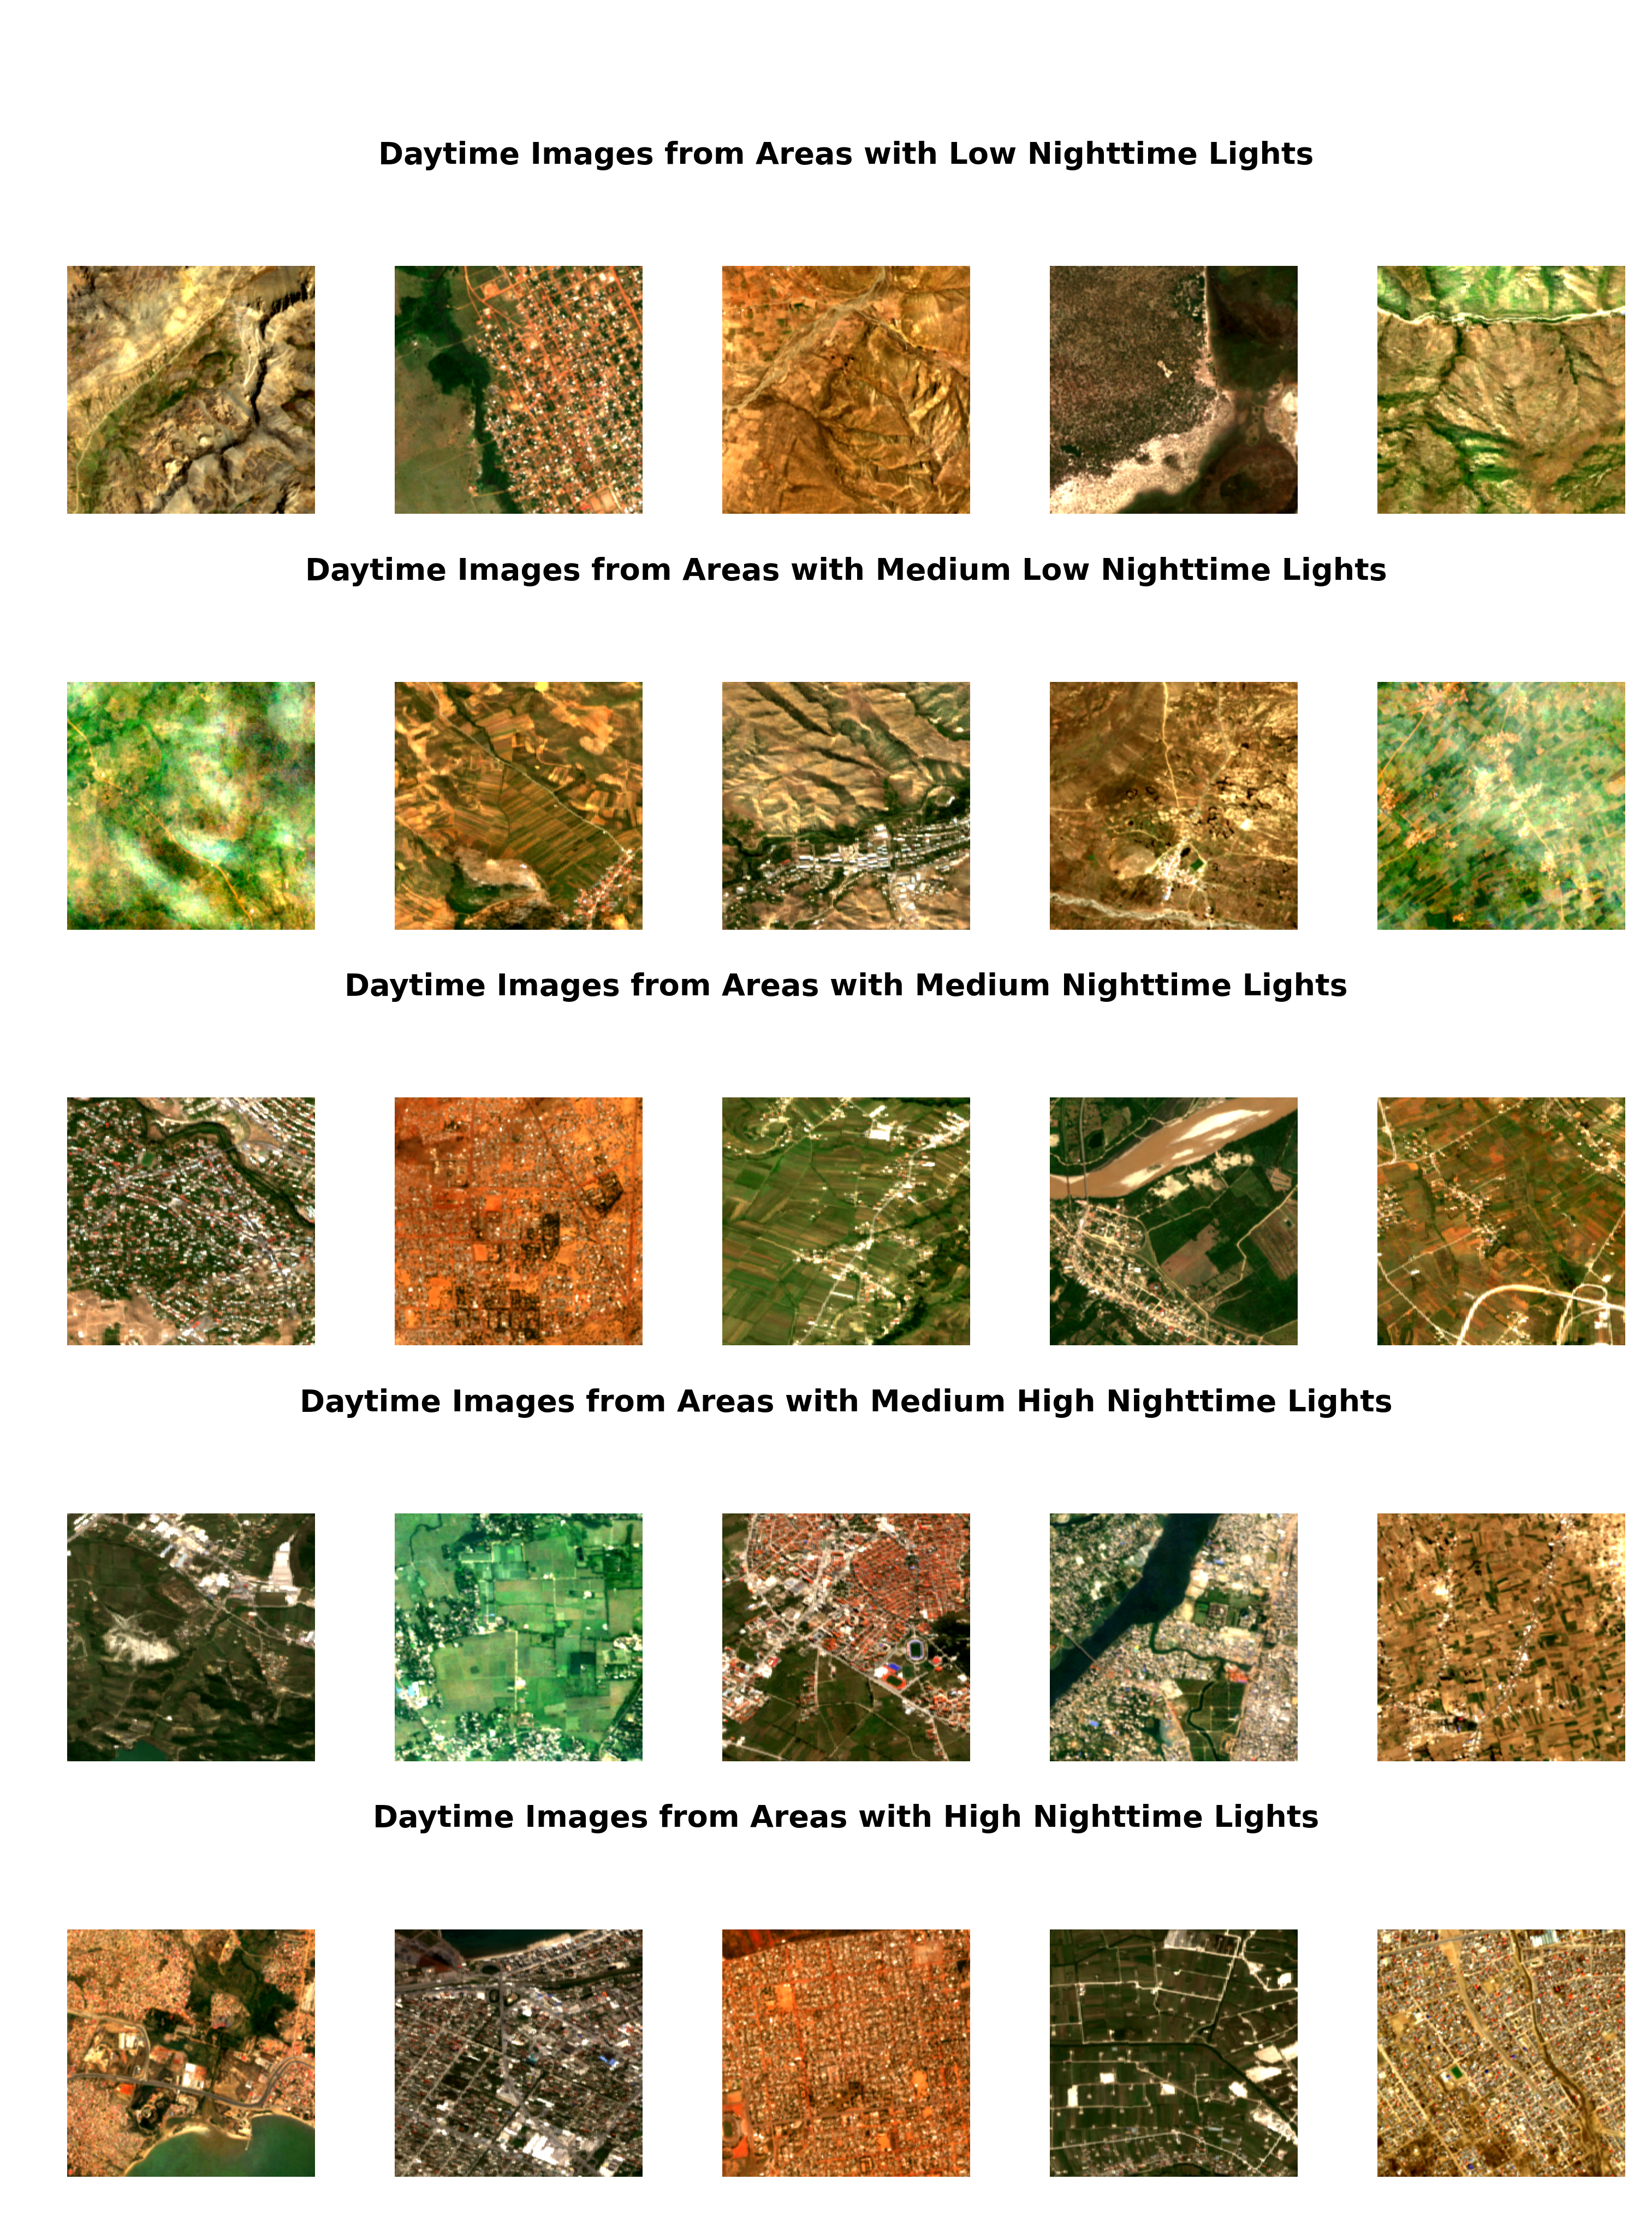
\includegraphics[width=1\textwidth]{figures/example_daytime_images.png}
    \caption{Example daytime images \textcolor{black}{from Sentinel-2 for} different nighttime lights groups\textcolor{black}{. The figure was produced using Python, version 3.9.13 (\url{https://www.python.org/}). Sentinel-2 data was queried using Google Earth Engine.}}
     \label{fig:example_daytime_images}
\end{figure}

\end{document}
